
\section{First class support for user defined types}

A necessary component to data abstraction is the concept of the {\em
first class} type.  A first class type, loosely defined, is one that
acts like any of the intrinsic types of a language.  This is to say
that a programmer can apply an intuitive set of assumptions when
he/she is using that type.

The relevance to data abstraction is the question of whether a
user-defined type is a first class type or not, and if not, how does
it act.  Programmers can feel more comfortable with types they know
are first class, because their intuitions about the use of intrinsic
types will carry over to their use of abstract first class types.  The
more a programmer has to know just what the specifics are about the
particular type he/she is manipulating, the more overhead he/she has
in using that type, and the less inclined he/she will be to abstract.

The concept of first class user-defined types remains controversial in
computer science.  For example, Java's intrinsic types are passed by
value, while its abstract types are passed by reference.  In this
case, the concept of first class type is immediately abandoned.  A
design goal in C++ was to give user-defined types first class status
by providing a uniform interface (in terms of constructors and
destructors) to the type syntax.  Perl
gives the programmer the means of defining types which have all the
properties of intrinsic types (though it neither encourages nor
discourages this practice).

It is not necessary that a language provide the means to make
user-defined first class types, because, despite such inconveniences,
it is possible that first class support can be had, if all users of
such types adopt a small set of global conventions.  This, {\em user
supported} first class data is the solution we have taken in Socorro.
While the FORTRAN standard itself does not support first class
user-defined types, we found a small set of conventions, adopted
uniformly across different user-defined types which makes our data
types all first class.

\subsection{What is a first class type (in FORTRAN)?}

FORTRAN provides intrinsic types to represent the primitive data types
found in most programming languages: integers, floats, and characters, all
with varying widths.  
Some of the more notable features of these types are:

\begin{enumerate}

\item Allocation and deallocation of the memory for local variables of
a first class type is automatic, i.e. their memory appears to be on
the stack.

\item The initialization of local variables of a first class type can
occur in their declarations, allowing procedure authors the ability to
guarantee that their data has some legitimate (or default) format
before they are used in the body of the procedure.

\item Arguments of a first class type to procedures (dummy variables)
are passed by reference, i.e. modifications made to them by the
called procedure are visible in the calling procedure.

\item Any first class type can be the type of a member of a data structure
(e.g. derived types).

\item Any first class type can be the return value of a function.

\end{enumerate}

While one might argue for the addition of other qualifications such as
assignment, equality testing, etc being added to this list, we will
emphasize the present list, as the support for other features can be
handled by appropriately written procedures (in fact, we strongly
suggest writing an assignment operator for every derived type, to
be sure that something sensible occurs when anyone does \verb+a=b+).

One immediately notes that FORTRAN allocatable arrays are not first
class types, for they may not be members of derived types, nor
returned by functions, even though the current FORTRAN standard allows
their storage to be automatically deallocated.  Arrays with the
\verb+pointer+ attribute instead of the \verb+allocable+ attribute
provide better fulfillment of the first class properties, but their
allocation and deallocation is not automatic, since they are heap
variables and not stack variables.

One also notes that derived types, without additional user
support, are not first class.  They cannot be initialized upon
declaration.  Additionally, it is a common desire for abstract types
to have some dynamically sized components.  Since this is only
achievable by having a member with the \verb+pointer+ attribute, such
derived types would be unable to automatically allocate and deallocate
these components.

Ultimately, what FORTRAN really lacks is a form of dynamic memory
which participates in some form of automatic garbage collection
\cite{Wilson.GCSurvey}.

\subsection{SADR: my,thy,glean,bequeath}

The trick we employ has been in the C/C++ programming literature for
some time, in the implementation of {\em smart pointers} (also called
{\em handles}, and sometimes {\em proxies} 
\cite{designpattterns,Coplien.AdvancedCPPIdioms}).
We have not seen it adapted for use with FORTRAN before.  The
convention employed will ensure that arbitrary user-defined types,
including those with dynamically sized components can all be treated
identically, and not much differently from intrinsic types.

Our goal is to, with minimal programmer overhead, provide a scalable
method of manipulating derived types with dynamic memory, with as much
ease as one manipulates intrinsic ``stack'' variables.

We adopted a programming convention, in which the use of all abstract
types is constrained by a small set of rules we call the {Scalable
Abstract Data Rules} (or SADR).  The SADR can be thought of as a
programming convention in which the user takes charge of
declaring just when and where he/she wants a variable to come in and
go out of scope, while the implementer of the type, writes functions
which will respond appropriately.

\begin{itemize}

\item Each abstract type has defined for it, the procedures
\verb+my+ (in two forms), \verb+thy+, \verb+glean+, and \verb+bequeath+.
The exact implementation of these procedures is only necessarily known
to the implementer of the type.

\item Each abstract type has at least one constructor function defined
for it, which is guaranteed to return a new valid representation of that
type.  The exact implementation of this function is only necessarily known
to the implementer of the type.

\item The programmer using that type must follow the conventions below
governing the use of the above special procedures whenever writing a
procedure which uses that type.

\end{itemize}

It is important to understand, that what is being presented here is an
interface for all abstract types and rules for programmers using
abstract types to always follow, even though the implementations of
these procedures will vary in complexity.

Let \verb+type(box_obj)+ be the abstract type under discussion.  The interface
and constraints are:

\begin{verbatim}
subroutine GLEAN(bx)
  type(box_obj) bx
\end{verbatim}
Gleaning is the central concept in this garbage collection scheme.  In
short, it means {\em finalizing what others do not want}.  If
\verb+bx+ is orphan (that is, no longer in any scope), glean finalizes
\verb+bx+, releasing whatever resources it should.  All SADR compliant
procedures will glean their arguments.

\begin{verbatim}
subroutine BEQUEATH(bx)
  type(box_obj) bx
\end{verbatim}
Should only be
called by a function returning \verb+type(box_obj)+.
Returns the function result, \verb+bx+, to the caller of that function.

\begin{verbatim}
subroutine MY(bx)
  type(box_obj) bx
\end{verbatim}
Called by a procedure to adopt the dummy variable \verb+bx+.  The
variable \verb+bx+ will not be is guaranteed not to be finalized 
by \verb+glean()+while it remains adopted.

(We overload \verb+my+ to have a one-argument and two-argument form)
\begin{verbatim}
subroutine MY(bx_init,bx)
  type(box_obj) bx
  type(box_obj), intent(in) :: bx_init
\end{verbatim}
Initializes the local variable \verb+bx+ with the value of the 
(initialized) variable \verb+bx_init+, declaring custody of
\verb+bx+.

\begin{verbatim}
function THY(bx) result(bxout)
  type(box_obj) bx, bxout
\end{verbatim}
Un-adopts the use of the variable \verb+bx+ and returns 
\verb+bx+ through \verb+bxout+.

(We adopt the convention of naming all constructor functions after the
data they construct.)
\begin{verbatim}
function box(arg1,arg2,arg3,...) result(bx)
  type(box_obj) bx
  [any type] arg1,arg2,arg3,....
\end{verbatim}
Returns a valid, orphan value of \verb+type(box_obj)+, based upon
the input arguments.

\subsubsection{Comparison with C++}

The SADR convention we propose can be thought of as an explicit
representation of the implicit calls to constructors and destructors
in C++, with some differences.  The C++ language supports abstract types
by compiling into procedures implicit calls to a {\em copy constructor}
for dummy variables, an {\em initialization constructor} for local
variables, at the beginning of the scope of a variable, and a 
{\em destructor} at the end of the scope of a variable.  Accordingly,
\verb+my+ is called upon entry into a scope, \verb+my+ is used
to initialize local variables, and \verb+glean(thy())+ is used to
send a variable out of scope and free its resources.

One interesting distinction between the user implemented SADR
convention and that C++ automatic constructor/destructor convention is
that a user can, and may find it efficient, to have a variable
leave the scope of a function abnormally early through a call to
another subroutine, (e.g. \\ \verb+ call do_next_thing(thy(bx))+).  Of
course, one could perform such tricks in C++ with some explicit
\verb+thy+ function and the adoption of a user convention.

\subsubsection{Quick tutorial}

One can identify three major modes for most, if not all, variables
in a FORTRAN program: local, dummy, and result variables.  In this
tutorial, we give examples of how Socorro abstract types are used in
all three modes.

For dummy variables, one uses the pattern:
\begin{verbatim}
subroutine f(bx)
  type(box_obj) bx

  call my(bx)
  ....
  <do things with bx>
  ....
  call glean(thy(bx))
end subroutine
\end{verbatim}
Variable \verb+bx+ is adopted to be used by \verb+subroutine f+.  Once
adopted, \verb+bx+ can be used within the body of \verb+subroutine f+.
The \verb+thy()+ function disowns \verb+bx+ and passes the result to
\verb+glean()+.  If (and only if) \verb+bx+ came into \verb+subroutine f+ as an orphan, it will enter \verb+glean+ as an orphan and
\verb+glean+ will finalize \verb+bx+.

For local variables, one uses the pattern:
\begin{verbatim}
subroutine f()
  type(box_obj) bx

  call my(box(1,2,3,4), bx)
  ....
  <do things with bx>
  ....
  call glean(thy(bx))
end subroutine
\end{verbatim}
Variable \verb+bx+ is initialized with a copy of the value 
of \verb+box(1,2,3,4)+, using the two-argument form of \verb+my+.
Once \verb+bx+ is
initialized, it may be used within the body of \verb+subroutine f+.
The \verb+thy()+ function disowns \verb+bx+ and passes the result
to \verb+glean()+.  \verb+bx+ is now orphan,
thus \verb+glean+ will finalize it.  

For result variables, one uses the pattern:
\begin{verbatim}
function f() result(bx)
  type(box_obj) bx

  call my(box(1,2,3,4),bx)
  ....
  <do things with bx>
  ....
  call bequeath(thy(bx))
end function
\end{verbatim}
Variable \verb+bx+ is initialized with
the value of \verb+box(1,2,3,4)+.   With \verb+bx+ 
initialized, it can be used within the body of \verb+function f+.
The \verb+thy()+ function un-adopts \verb+bx+
and passes the result to \verb+bequeath()+ which returns an
orphan value of \verb+type(box_obj)+ to the caller of 
\verb+function f+.

One may wonder what gleaned the result of \verb+box(1,2,3,4)+ in the
last two examples.  The full explanation is in the advanced SADR
tutorial.  The short answer is that all functions glean their dummy
arguments, and that goes for the first argument of the two-argument 
\verb+my+ too.

{\bf Important:} we believe that reader should note the distinction
between using the two-argument \verb+my()+ for initialization and
using assignment for initialization.  According to the current FORTRAN
standard, an overloaded assignment statement,\\
\verb+  a = b+\\
is equivalent to the statement\\
\verb+  call assign_abtype(a,b)+\\
for some user defined \verb+assign_abtype+ subroutine.  It is
further specified that \verb+assign_abtype+ must have 
\verb+intent(inout)+ on \verb+a+ and \verb+intent(in)+ on \verb+b+.
Thus, it is implicitly assumed that \verb+a+ already has
an initial value, i.e. that its bit-patterns are in the format
of some valid data of \verb+type(abtype)+.  Therefore, the \verb+=+-sign,
is not applicable for the initialization of abstract data:\\
\verb+  type(abtype)   a = b+\\
Some compilers may reduce this to
\begin{verbatim}
  type(abtype)   a
  call assign_abtype(a,b)
\end{verbatim}
but this is problematic (any inquiries \verb+assign_abtype+ makes
into \verb+a+ would have an unspecified result).  Thus, the two-argument
form of the generic \verb+my+ function must be called on any uninitialized
data before any use or inquiries of the data are made.  For example:
\begin{verbatim}
  type(abtype)   a
  call my(b,a)
\end{verbatim}

\subsubsection{Quick advanced tutorial}

While one can never go wrong with the three implementations
above, there are optimizations which a skilled user might
wish to make in his application of the SADR, which eliminate
one or more procedure invocations.

The most substantial optimizations concern the use of dummy variables:
\begin{verbatim}
subroutine f(bx)
  type(box_obj) bx

  call my(bx)
  ....
  <do stuff to bx>
  ....
  call g(thy(bx))
  ....
  <do nothing with bx>
  ....
end subroutine
\end{verbatim}
In this case, the subroutine makes use of \verb+subroutine g+
instead of \verb+glean+ when it un-adopts \verb+bx+.
Since all compliantly written procedures finalize their orphan
arguments, \verb+subroutine g+ will glean \verb+bx+.

Alternatively,
\begin{verbatim}
subroutine f(bx)
  type(box_obj) bx

  ....
  <do stuff to bx>
  ....
  call g(bx)
  ....
  <do nothing with bx>
  ....
end subroutine
\end{verbatim}
In this case the subroutine never makes use of \verb+bx+, as above,
except in passing \verb+bx+ on, only once, to \verb+subroutine g+.
Thus, it does not need to adopt and then un-adopt \verb+bx+.

Finally,
\begin{verbatim}
subroutine f(bx)
  type(box_obj) bx

  ....
  <do nothing to bx>
  ....
  call glean(bx)
end subroutine
\end{verbatim}
In this case the subroutine never makes use of \verb+bx+, thus
its use never needs to be adopted (with \verb+my+) and then
un-adopted (with \verb+thy+).  \verb+bx+ is passed straight on
to \verb+glean+.

\subsection{SADR implementations}

The SADR rules are designed to encompass abstract types with differing
levels of sophistication.  In Socorro, there are three such levels:
fixed size values, variable size values, and lazy copied values (in
increasing order of complexity).  We sketch the implementation of
these types in what follows, and give some discussion of two other
variants which are not currently found in the Socorro code: handles,
and handles with lazy copied values.

Note: in all the examples below, the members of \verb+type(box_obj)+
are all private.  This is a result of the need for some members to
be private and the lack of the current FORTRAN standard to provide
a means of selectively applying the \verb+private+ attribute.
We are told this will be fixed in the next revision of the standard.

The implementations below are unique, or the most efficient.  They
have been chosen primarily for illustrative purposes, being the most
straightforward version we could think of.

\subsubsection{Fixed size value}

In this case, \verb+type(box_obj)+ is some fixed size derived type
like:

\begin{verbatim}
type, public:: box_obj
private
  integer height,width,area
end type box_obj
\end{verbatim}

Of course, such a simple derived type is almost a first class
type already in FORTRAN, so there is little that one needs to
do to implement the SADR.

\begin{verbatim}
subroutine glean(bx)
  type(box_obj) bx
  continue
end subroutine glean

subroutine bequeath(bx)
  type(box_obj) bx
  continue
end subroutine bequeath

interface my
  module procedure my_1arg, my_2arg
end interface my

subroutine my_1arg(bx)
  type(box_obj) bx
  continue
end subroutine my_1arg

subroutine my_2arg(bx_init,bx)
  type(box_obj) bx
  type(box_obj), intent(in) :: bx_init
  bx = bx_init
end subroutine my_2arg

function thy(bx) result(bx_out)
  type(box_obj) bx
  type(box_obj) bx_out
  bx_out = bx
end function thy

function box(h,w) result(bx)
  integer, intent(in) :: h,w
  type(box_obj) bx
  bx%height = h
  bx%width = w
  bx%area = h*w
end function box

\end{verbatim}

In this case, the default assignment operation produces reasonable
behavior, so we do not need to supply one.

\subsubsection{Variable size value}

In this case, \verb+type(box_obj)+ could be some fixed size derived type
like:

\begin{verbatim}
type, public:: box_obj
private
  integer ref
  integer height,width
  real, pointer :: area(:,:)
end type box_obj
\end{verbatim}

Here we see the first example of an abstract type which has a
dynamically allocated component.  In order to behave like first class
data, this type must be able to deallocate this component when it is
no longer in anyone's scope.  We have placed a reference count in the
implementation of \verb+type(box_obj)+.  This reference count should
always be a private member of the abstract type.

\begin{verbatim}
subroutine glean(bx)
  type(box_obj) bx
  if (bx%ref<1) deallocate(bx%area)
end subroutine glean

subroutine bequeath(bx)
  type(box_obj) bx
  continue
end subroutine bequeath

interface my
  module procedure my_1arg, my_2arg
end interface my

subroutine my_1arg(bx)
  type(box_obj) bx
  bx%ref = bx%ref+1   ! adopts
end subroutine my_1arg

subroutine my_2arg(bx_init,bx)
  type(box_obj) bx
  type(box_obj), intent(in) :: bx_init
  bx%ref = 1      ! declares initial custody
  bx = bx_init
end subroutine my_2arg

function thy(bx) result(bx_out)
  type(box_obj) bx
  type(box_obj) bx_out
  bx_out%ref = bx%ref -1  ! unadopts
  bx%ref = 0   ! to make assignment swing pointer, not copy data
  bx_out = bx
  bx%ref = bx_out%ref ! restore the ref in bx
end function thy

function box(h,w) result(bx)
  integer, intent(in) :: h,w
  type(box_obj) bx
  bx%height = h
  bx%width = w
  allocate(bx%area(h,w))
  bx%area = 0.0
  bx%ref = 0       ! make orphan
end function box

subroutine assign_box(bx,bx_in)
  type(box_obj),intent(inout) :: bx
  type(box_obj),intent(in) :: bx_in
  real, pointer :: atmp(:,:)
  bx%height = bx_in%height
  bx%width = bx_in%width
  if (bx_in%ref<1) then  ! don't copy if bx_in is orphaned
    deallocate(bx%area)
    bx%area => bx_in%area
  else
    allocate(atmp(bx_in%height,bx_in%width)) ! create temp
    atmp = bx_in%area     ! copy source to the temp
    deallocate(bx%area)   ! clean up destination
    bx%area => atmp       ! swing dest pointer to temp
  end if
end subroutine assign_box

\end{verbatim}

In this case, the default assignment operation does not produce
reasonable behavior, since two different boxes should have distinct
data allocated for their area members, so that modifications to
one does not affect the other.

The \verb+%ref+ member of this version of \verb+type(box_obj)+ is a
running count of how many valid identifiers exist for the data in a
given instance.  With the call-by-reference semantics of the FORTRAN
language, this is often just the current stack depth, relative to
the point at which the variable is declared (though examples can
be easily contrived where it is not).

\subsubsection{Handles}

\label{handlesec}

Handles are an easy way to avoid unnecessary copying.  In short, the
data type becomes a small fixed-size reference to a large node of
allocated data which represents the value of the handle (see figure
\ref{handlefig}).

\begin{figure}
\begin{center}
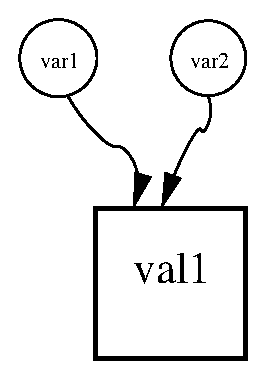
\epsfig{file=figs/handle.eps}
\caption{variables as handles to data}
\label{handlefig}
\end{center}
\end{figure}

We define \verb+type(box_obj)+ in terms of two types, one of which is
private:

\begin{verbatim}
type, public:: box_obj
private
  integer ref
  type(box_rep), pointer :: o
end type box_obj

type, private:: box_rep   ! defines a value node
private
  integer ref
  integer height,width
  real, pointer :: area(:,:)
end type box_rep
\end{verbatim}

\verb+type(box_obj)+ is the only type that users of the box
module can declare.  But it contains little more than a pointer
to a value.  The user does not have to know that he/she has only a
very lightweight reference.

The reference count in \verb+type(box_obj)+ counts just what it did
before, the number of valid identifiers for the variable, while the
reference count in \verb+type(box_rep)+ counts the total number of
valid identifiers for the data.

Copying is minimized by exploiting the fact that several different
variables of \verb+type(box_obj)+ might all have the same value,
consolidated in a single value node.  Copying does not occur at
assignment.  Instead, assignment merely binds the reference to another
value node.  When all the handles for a given value are gone, the
value deallocates itself.

\begin{verbatim}
subroutine glean(bx)
  type(box_obj) bx
  if (bx%o%ref<1) then
    deallocate(bx%o%area)  ! get rid of data
    deallocate(bx%o)       ! get rid of node
  end if
end subroutine glean

subroutine bequeath(bx)
  type(box_obj) bx
  continue
end subroutine bequeath

interface my
  module procedure my_1arg, my_2arg
end interface my

subroutine my_1arg(bx)
  type(box_obj) bx
  bx%ref = bx%ref+1      ! adopts
  bx%o%ref = bx%o%ref+1  ! number of node users increases too
end subroutine my_1arg

subroutine my_2arg(bx_init,bx)
  type(box_obj) bx
  type(box_obj), intent(in) :: bx_init
  bx%o => bx_init%o   ! just swing the pointer
  bx%ref = 1          ! declare initial custody of the box_obj
  bx%o%ref = bx%o%ref+1   ! increase number using the box_rep
end subroutine my_2arg

function thy(bx) result(bx_out)
  type(box_obj) bx
  type(box_obj) bx_out
  bx%ref = bx%ref -1     ! un-adopt
  bx%o%ref = bx%o%ref -1 
  bx_out%ref = bx%ref    ! create return value
  bx_out%o => bx%o
end function thy

function box(h,w) result(bx)
  integer, intent(in) :: h,w
  type(box_obj) bx
  allocate(bx%o)      ! make a new value node
  bx%o%height = h
  bx%o%width = w
  allocate(bx%o%area(h,w))
  bx%o%area = 0.0
  bx%ref = 0       ! make orphan
  bx%o%ref = 0
end function box

subroutine assign_box(bx,bx_in)
  type(box_obj),intent(inout) :: bx
  type(box_obj),intent(in) :: bx_in
  type(box_obj) bx_tmp
  bx_tmp%o => bx%o    ! may need to glean up the old value
  bx%o%ref = bx%o%ref - bx%ref  ! swing pointer and move ref's
  bx%o => bx_in%o
  bx%o%ref = bx%o%ref + bx%ref
  call glean(bx_tmp) 
  call glean(bx_in)
end subroutine assign_box

\end{verbatim}

One shortcoming of this form of data is that it no longer
follows the semantics of the previous types.  Consider, the following
procedures, which might be implemented in the box module:

\begin{verbatim}
function sum_area(bx) result(ans) ! a non-mutating procedure
  real ans
  type(box_obj), intent(inout) :: bx
  call my(bx)
  ans = sum(bx%o%area)
  call glean(thy(bx))
end function sum_area

subroutine normalize(bx)       ! an example of a mutating procedure
  type(box_obj), intent(inout) :: bx
  call my(bx)
  bx%o%area = bx%o%area - sum(bx%o%area)/size(bx%o%area)
  call glean(thy(bx))
end subroutine normalize
\end{verbatim}

The first does nothing more than read values from the node.
However, the second function modifies the value of its
argument by modifying the underlying value node.  The existence
of such a procedure, or {\em mutator}, can lead to such
counter-intuitive situations such as:
\begin{verbatim}
  print *,sum_area(bbox)       ! prints out ``1.0d0''
  abox = bbox
  print *,sum_area(abox)       ! prints out ``1.0d0''
  call normalize(abox)
  print *,sum_area(abox)       ! prints out ``0.0d0''
  print *,sum_area(bbox)       ! prints out ``0.0d0''
\end{verbatim}

Whenever either \verb+abox+ or \verb+bbox+ is mutated, the values of
both appear to change.  Instead of following {\em value semantics},
as first class types do, handles follow {\em pointer semantics}.

In order to have a separate copy that will not affect the rest,
a new function needs to be introduced.
\begin{verbatim}
subroutine fork(bx)              ! for coping handles
  type(box_obj) bx
  type(box_rep), pointer :: node
  if (bx%o%ref>bx%ref) then      ! if bx doesn't own the node
    allocate(node)               ! make a new node
    node%ref = 0
    allocate(node%area(bx%o%height,bx%o%width))
    node%area = bx%o%area       ! copy allocated stuff
    node%height = bx%o%height   ! copy unallocated stuff
    node%width = bx%o%width
    bx%o%ref = bx%o%ref - bx%ref    ! swing pointers
    bx%o => node
    bx%o%ref = bx%o%ref + bx%ref
  end if
  glean(bx)
end subroutine fork
\end{verbatim}

\begin{figure}
\begin{center}
\begin{enumerate}
\item 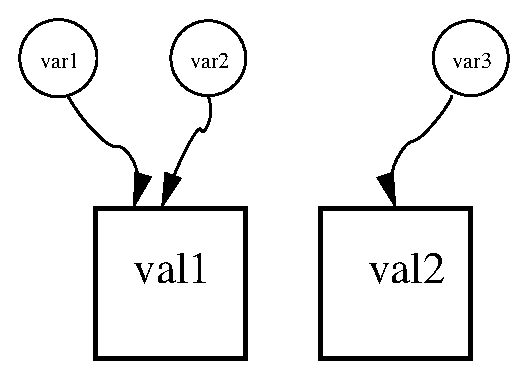
\epsfig{file=figs/share.eps}
\item 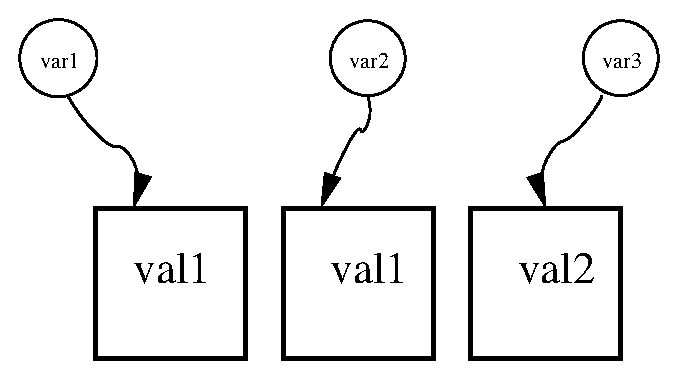
\epsfig{file=figs/fork.eps}
\end{enumerate}
\caption{Before a fork (1), after a fork (2)}
\label{forkfig}
\end{center}
\end{figure}

This subroutine checks whether its input shares its value with
anyone else, and if so, makes a new node of which its input will now
have sole custody (see figure \ref{forkfig}).  
Now the example above can be
modified slightly using \verb+fork+:
\begin{verbatim}
  print *,sum_area(bbox)       ! prints out ``1.0d0''
  abox = bbox 
  call fork(abox)              ! ensure independence of abox
  print *,sum_area(abox)       ! prints out ``1.0d0''
  call normalize(abox)
  print *,sum_area(abox)       ! prints out ``0.0d0''
  print *,sum_area(bbox)       ! prints out ``1.0d0''
\end{verbatim}

The \verb+fork+ constructor, or some similar procedure, allows the
user to establish the independence of \verb+abox+ before modifying it.
In the Java language, where abstract types are (second class) handles,
forking is done by a routine called \verb+clone()+ (e.g. 
\verb+a = b.clone()+).

One appealing alternative syntax to the \verb+fork+ subroutine is
a \verb+box_fork+ constructor (overloading the generic \verb+box+
constructor function), which can be expressed in terms of \verb+fork+
as:
\begin{verbatim}
interface box
  module procedure box_fork
end interface

function box_fork(bx) result(newbx)
  type(box_obj), intent(in) :: bx
  type(box_obj) newbx
  call my(bx,newbx)
  call fork(newbx)
  call bequeath(thy(newbx))
end function box_fork
\end{verbatim}
Its appeal is primarily in the fact that it adds no new procedure names
to the SADR, while giving users the ability fork efficiently.

Handles can be a convenience, but they are counter to
the intuition of the typical FORTRAN programmer.  Additionally, they
can be a serious vulnerability to a software component that needs to
share important, large, pieces of data with other components, yet does
not want to give everyone a license to modify its internal state.
As such, we have not included any handles in the Socorro code.


\subsubsection{Lazy copied values}

\label{lazysec}

Lazy copying is an optimization which prevents excessive copying
that might occur with simple variable size value types, while
still retaining value semantics.  Thus, the user need never
know that he/she is using anything but a first class type.

We define a lazy copied \verb+type(box_obj)+ as a modification of
the handle version of \verb+type(box_obj)+.
With identical implementations of 
\verb+glean+, \verb+bequeath+, \verb+my+, \verb+thy+, and
\verb+assign_box+.  

To create the illusion of regular copying,
the \verb+fork+ subroutine is made private, only callable by functions
in the box module.  The implementer must also identify and modify
every mutator of \verb+type(box_obj)+ to call \verb+fork+ before acting.
\begin{verbatim}
subroutine normalize(bx)    ! a mutating procedure
  type(box_obj), intent(inout) :: bx
  call my(bx)
  call fork(bx)             ! make sure you own the node
  bx%o%area = bx%o%area - sum(bx%o%area)/size(bx%o%area)
  call glean(thy(bx))
end subroutine
\end{verbatim}

The result is a data type that performs like a handle behind the
scenes, copying around lightweight references instead of heavyweight
data.  However, any time a mutator is called, one is assured that it
will happen only on ones own value, since a copy will automatically
occur if the value is shared (this policy is also called
{\em copy on write}).
\begin{verbatim}
  print *,sum_area(bbox)       ! prints out ``1.0d0''
  abox = bbox
  print *,sum_area(abox)       ! prints out ``1.0d0''
  call normalize(abox)
  print *,sum_area(abox)       ! prints out ``0.0d0''
  print *,sum_area(bbox)       ! prints out ``1.0d0''
\end{verbatim}

This type allows for large quantities of data to be shared by
many different components of a program, just as handles do, but
insulates the owner of that data from any tampering from outsiders,
unlike handles.

Lazy copied values are used extensively in the Socorro code to share data
between software components.

\subsubsection{Handles with lazy copied values}

The techniques described so far can be scaled up in a number of ways
implementing a variety of memory management policies.  Here we present
an example that the astute reader might have anticipated.

With one level of indirection, one can diminish the need for excessive
copying, using handles or lazy copied values.  With two levels of
indirection, more sophisticated memory management is possible.  One
structure looks like it might have promise, but which did not find its
way into the current Socorro code is that of handle with a lazy copied
value.  This can be thought of as a handle, that has a lazy
\verb+fork+ command.

This can be achieved by combining the lazy copied type
\verb+type(box_obj)+ described in Section \ref{lazysec}, with the
handle construction of Section \ref{handlesec}.

\begin{verbatim}
type, public:: box_obj    ! a handle with a lazy copied value
private
  integer ref
  type(box_laz), pointer :: o
end type box_obj

type, private:: box_laz    ! a lazy copied value node
private
  integer ref
  type(box_rep), pointer :: o
end type box_laz

type, private:: box_rep   ! defines a value node
private
  integer ref
  integer height,width
  real, pointer :: area(:,:)
end type box_rep
\end{verbatim}

\begin{figure}
\begin{center}
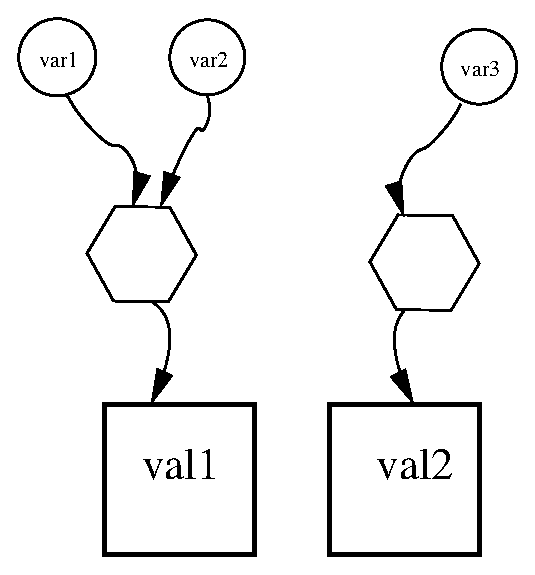
\epsfig{file=figs/complex.eps}
\caption{Additional layer allows for both handle and lazy copying}
\label{complexfig}
\end{center}
\end{figure}

This causes a three-level structure shown in figure \ref{complexfig}
(with the intermediate \verb+type(box_laz)+ represented with
hexagons).  The ref count in \verb+type(box_obj)+ counts the number of
valid identifiers for this variable.  The ref count in
\verb+type(box_laz)+ counts total number of the number of identifiers
using this lazy value.  The ref count in \verb+type(box_rep)+ counts
the number of identifiers using this node value.  In this
implementation.

\begin{verbatim}
subroutine glean(bx)
  type(box_obj) bx
  if (bx%o%o%ref<1) then
    deallocate(bx%o%o%area)  ! get rid of data
    deallocate(bx%o%o)       ! get rid of node
  end if
  if (bx%o%ref<1) then
    deallocate(bx%o)         ! get rid of lazy node
  end if
end subroutine glean

subroutine bequeath(bx)
  type(box_obj) bx
  continue
end subroutine bequeath

interface my
  module procedure my_1arg, my_2arg
end interface my

subroutine my_1arg(bx)
  type(box_obj) bx
  bx%ref = bx%ref+1      ! adopts
  bx%o%ref = bx%o%ref+1  ! number of node users increases too
  bx%o%o%ref = bx%o%o%ref+1
end subroutine my_1arg

subroutine my_2arg(bx_init,bx)
  type(box_obj) bx
  type(box_obj), intent(in) :: bx_init
  bx%o => bx_init%o   ! just swing the pointer
  bx%ref = 1          ! declare initial custody of the box_obj
  bx%o%ref = bx%o%ref+1   ! increase number using the nodes
  bx%o%o%ref = bx%o%o%ref+1
end subroutine my_2arg

function thy(bx) result(bx_out)
  type(box_obj) bx
  type(box_obj) bx_out
  bx%ref = bx%ref -1     ! un-adopt
  bx%o%ref = bx%o%ref -1 
  bx%o%o%ref = bx%o%o%ref -1 
  bx_out%ref = bx%ref    ! create return value
  bx_out%o => bx%o
end function thy

function box(h,w) result(bx)
  integer, intent(in) :: h,w
  type(box_obj) bx
  allocate(bx%o)      ! make a new lazy node
  allocate(bx%o%o)      ! make a new value node
  bx%o%o%height = h
  bx%o%o%width = w
  allocate(bx%o%o%area(h,w))
  bx%o%o%area = 0.0
  bx%ref = 0       ! make orphan
  bx%o%ref = 0
  bx%o%o%ref = 0
end function box

subroutine assign_box(bx,bx_in)
  type(box_obj),intent(inout) :: bx
  type(box_obj),intent(in) :: bx_in
  type(box_obj) bx_tmp
  bx_tmp%o => bx%o    ! may need to glean up the old value
  bx%o%ref = bx%o%ref - bx%ref  ! swing pointer and move ref's
  bx%o%o%ref = bx%o%ref - bx%o%ref
  bx%o => bx_in%o
  bx%o%ref = bx%o%ref + bx%ref
  bx%o%o%ref = bx%o%o%ref + bx%ref
  call glean(bx_tmp) 
  call glean(bx_in)
end subroutine assign_box

subroutine fork(bx)              ! for copying lazy nodes
  type(box_obj) bx
  type(box_laz), pointer :: node
  if (bx%o%ref>bx%ref) then      ! if bx doesn't own lazy node
    allocate(node)               ! make a new lazy node
    node%ref = 0
    node%o => bx%o%o             ! point lazy node to value node
    bx%o%ref = bx%o%ref - bx%ref    ! swing pointers
    bx%o => node
    bx%o%ref = bx%o%ref + bx%ref    ! don't need to change %o%o%ref's
  end if
  glean(bx)
end subroutine fork

subroutine, private :: val_fork(bx) ! the lazy node fork
  type(box_obj) bx
  type(box_rep), pointer :: node
  if (bx%o%o%ref>bx%o%ref) then  ! if lazy node doesn't own value
    allocate(node)               ! make a new value
    node%ref = 0
    allocate(node%area(bx%o%o%height,bx%o%o%width))
    node%area = bx%o%o%area       ! copy allocated stuff
    node%height = bx%o%o%height   ! copy unallocated stuff
    node%width = bx%o%o%width
    bx%o%o%ref = bx%o%o%ref - bx%o%ref    ! swing lazy node's pointers
    bx%o%o => node
    bx%o%o%ref = bx%o%o%ref + bx%o%ref
  end if
  glean(bx)
end subroutine val_fork

\end{verbatim}

One notices two forks, a public one which forks the obj/laz connection
and a private one which forks the laz/rep connection (see figures
\ref{complexforkfig} and \ref{complexfork2fig}).

\begin{figure}
\begin{center}
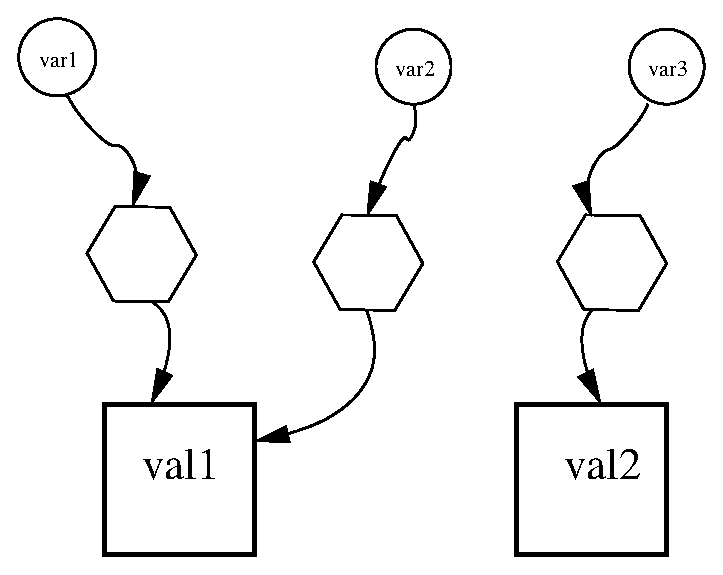
\epsfig{file=figs/complexfork.eps}
\caption{Forking a handle simply creates a new lazy-copied value}
\label{complexforkfig}
\end{center}
\end{figure}

\begin{figure}
\begin{center}
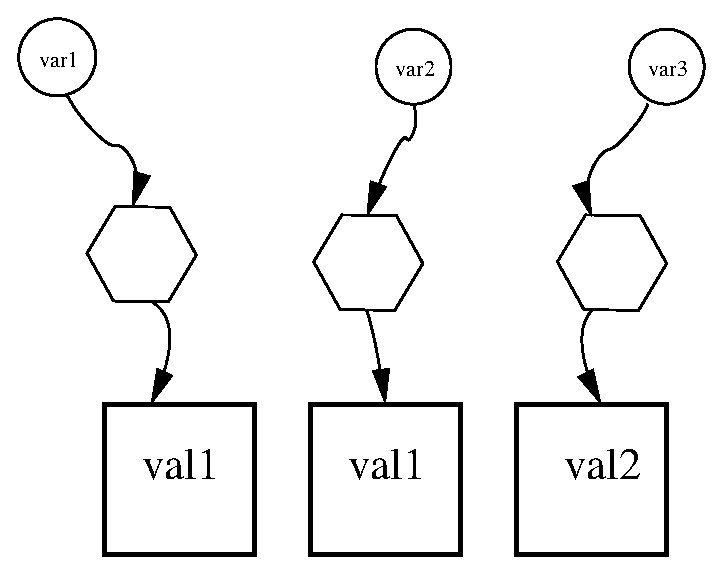
\epsfig{file=figs/complexfork2.eps}
\caption{Mutating a handle forks the node value}
\label{complexfork2fig}
\end{center}
\end{figure}

When the user calls \verb+fork+, a new lazy node is spawned, but no
large copying takes place.  Meanwhile, the implementer of the box abstraction
must use \verb+val_fork+ in order to give the illusion of lazy copying.

In the \verb+normalize+ example:
\begin{verbatim}
subroutine normalize(bx)    ! a mutating procedure
  type(box_obj), intent(inout) :: bx
  call my(bx)
  call val_fork(bx)          ! make sure lazy node owns the value
  bx%o%o%area = bx%o%o%area - sum(bx%o%o%area)/size(bx%o%o%area)
  call glean(thy(bx))
end subroutine
\end{verbatim}

The user does not see a difference between using this type and the
handle type.
\begin{verbatim}
  print *,sum_area(bbox)       ! prints out ``1.0d0''
  abox = bbox; call fork(abox)
  cbox = bbox; call fork(cbox) ! abox,bbox,cbox now have the same 
                               ! value node and differing lazy nodes
  print *,sum_area(abox)       ! prints out ``1.0d0''
  call normalize(abox)         ! value node copy for abox
                               ! bbox, cbox still have same value nodes
  print *,sum_area(abox)       ! prints out ``0.0d0''
  print *,sum_area(bbox)       ! prints out ``1.0d0''
  print *,sum_area(cbox)       ! prints out ``1.0d0''
  call normalize(cbox)         ! value node copy for cbox
  print *,sum_area(bbox)       ! prints out ``1.0d0''
  print *,sum_area(cbox)       ! prints out ``0.0d0''
\end{verbatim}
However, from a performance standpoint, only one substantial copy
occurs at the point where \verb+abox+ or \verb+cbox+ are mutated.
Where the regular handle implementation decreases copying by
sharing values, the only way to protect the data in one handle from
being mutated by actions on another handle is to call \verb+fork+
which is implemented by copying.  In this implementation, the
call to \verb+fork+ is implemented via lazy copying, so the data
is protected, without necessarily incurring substantial copying
expense until an attempt is made to mutate the \verb+fork+-ed handle.

Handles with lazy copied values, would seem to be an ideal way for
software components to both protect their data and allow portions
of their data to be modified by outside components.  Like handles,
however, they do not behave like first class types, and would
therefore be counter-intuitive to FORTRAN programmers, so we have
yet to implement them in Socorro.

We should also comment that in languages with support for indirection
and overloaded indirection, like C++ or Perl, one could implement
a handle with lazy copied values as a simple extension of a lazy copied value
type, having both the lazy type and the handles to the lazy type 
coexisting and sharing code.  This is not so easy in FORTRAN unfortunately.

\subsection{Memory management and scaling}

One important point left to be discussed about the SADR rules is how
they scale in a data hierarchy.  The design of the interface went
through a couple iterations, for it was found that some versions,
which worked fine for types with intrinsic members, could not easily
be applied to higher level types with their own garbage collected members.

A prototypical higher-order (lazy copied) type could be defined as follows:
\begin{verbatim}
    type, public :: high_obj
    private
      integer ref
      type(high_rep), pointer :: o
    end type

    type, public :: high_rep
    private
      integer  ref
      type(low_obj)  :: mem   ! note member is a SADR type
      real*8 other
    end type

    subroutine glean(h)
      type(high_obj) h
      if (h%o%ref<0) then
        call glean(h%mem)
        deallocate(h%o)
      end if
    end subroutine

    subroutine bequeath(h)
      type(high_obj) h
      continue
    end subroutine

    subroutine my_1arg(h)
      type(high_obj) h
      h%ref = h%ref +1
      h%o%ref = h%o%ref +1
    end subroutine

    subroutine my_2arg(hin,hout)
      type(high_obj) hin,hout
      hout%ref = 1
      hout%o => hin%o
      hout%o%ref = hout%o%ref +1
    end subroutine

    function thy(h) result(hout)
      type(high_obj) h,hout
      h%ref = h%ref -1
      h%o%ref = h%o%ref -1
      hout%ref = h%ref
      hout%o => h%o%ref
    end function

    function high(l,ot) result(h)
      type(high_obj) h
      type(low_obj), intent(in) ::l
      real*8, intent(in) :: ot
      h%ref = 0
      allocate(h%o)
      h%o%ref = 0
      call my(l,l%o%mem)
      h%o%other = ot**2
    end
\end{verbatim}

We see that it is only necessary to \verb+my+ the \verb+%mem+
member of \verb+type(high_obj)+ once upon creation and to \verb+thy+
it just once when \verb+type(high_obj)+ is being deconstructed by
\verb+glean+.  Another way to say this is membership in another value
counts as one reference.  In doing so, we avoid the need to traverse
all the data members of the higher type recursively (for a complicated
data structure this would be unnecessarily expensive).

The reader will also notice that because constructors are
functions, one need not declare intermediate results just to
initialize a higher-order data type.  The initialization of
\verb+h+ of type \verb+type(high_obj)+,
\begin{verbatim}
      type(low_obj)  tmp
      ....
      call my(low(1,2,3), tmp)   ! initialize a temporary
      call my(high(tmp,9),  h)   ! initialize h
      call glean(thy(tmp))       ! get rid of temp
      ....
\end{verbatim}
can be optimized to
\begin{verbatim}
      ....
      call my(high(low(1,2,3),9.0d0),h)
      ....
\end{verbatim}
saving three unnecessary lines of program text as well as being
more memory efficient if real copies are done in the initialization.
If \verb+type(low_obj)+ also has a SADR member, there would be
three more unnecessary lines in the first pattern.
In fact, the first construction pattern has three unnecessary lines of 
text for every SADR type which requires initialization, that
would add about fifteen unnecessary lines to the initialization
of Socorro's \verb+type(config_obj)+.  For this reason,
we caution anyone serious
about creating hierarchical data not to adopt the sort of
\verb+call new()+ and \verb+call delete()+ syntax which has been
suggested in \cite{KimLeeMartin.OORI,DecykNotronSzymanski.OOF90}

Finally, we present an example of a fork routine which minimizes
copying in a hierarchy.  Let's us suppose that \verb+type(high_obj)+
and \verb+type(low_obj)+ are to be lazy copied values.  The fork
would be
\begin{verbatim}
subroutine fork(h)              ! for coping handles
  type(high_obj) h
  type(high_rep), pointer :: node
  if (h%o%ref>h%ref) then      ! if h doesn't own the node
    allocate(node)               ! make a new node
    node%ref = 0
    call my(h%o%mem,node%mem)    ! (lazy) copy value
    node%other = h%o%other       ! copy value
    h%o%ref = h%o%ref - h%ref    ! swing pointers
    h%o => node
    h%o%ref = h%o%ref + h%ref
  end if
  glean(h)
end subroutine fork
\end{verbatim}
where one notes that there is not nor needs to be any recursive call
to low's \verb+fork()+ procedure (which should be private anyhow).
Since only lazy copying is performed on the members, no 
lazy copied member is
really copied on the fork until that member is modified (see figure
\ref{lch}).

\begin{figure}
\begin{center}
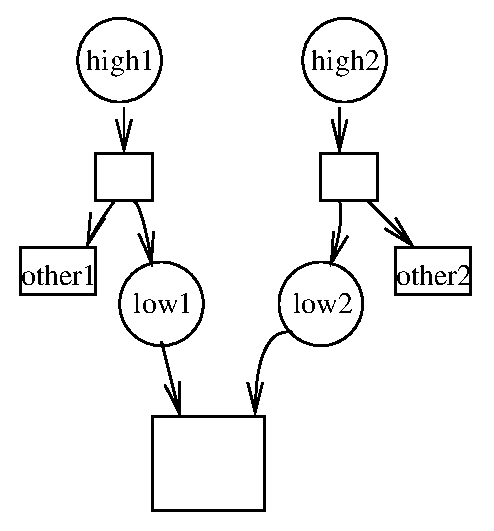
\epsfig{file=figs/lc_hierarchy.eps}
\caption{Example of lazy copying in a hierarchy}
\label{lch}
\end{center}
\end{figure}

In complicated hierarchies, this allows copying to be avoided
separately for each member of the complex (see figure \ref{biglch}).
\begin{figure}
\begin{center}
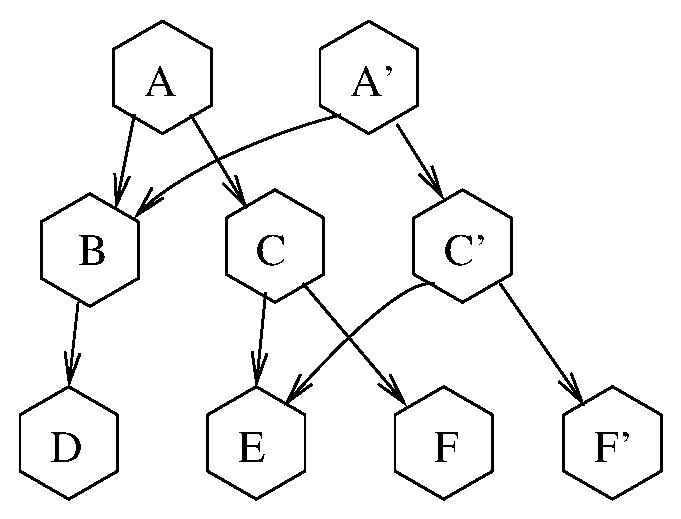
\epsfig{file=figs/biglc_hierarchy.eps}
\caption{Example of lazy copying in a complicated hierarchy (condensing
different abstract types into hexes).  This results from copying 
A and modifying F.}
\label{biglch}
\end{center}
\end{figure}
This keeps real copying to a minimum.
